\documentclass[12pt,a4paper]{article}

% =====================================================================
% PAQUETES
% =====================================================================
\usepackage[utf8]{inputenc}
\usepackage[T1]{fontenc}
\usepackage[english]{babel}


% Matemáticas
\usepackage{amsmath}
\usepackage{amssymb}
\usepackage{amsfonts}
\usepackage{mathtools}

% Unidades SI
\usepackage{siunitx}
\sisetup{
  per-mode        = symbol,
  detect-all,
  output-decimal-marker = {,},
  group-separator = {.},
  group-minimum-digits = 4
}

% Gráficos y color
\usepackage{graphicx}
\usepackage{xcolor}
\usepackage{tcolorbox}
\tcbuselibrary{skins, breakable}

% Tablas
\usepackage{booktabs}
\usepackage{tabularx}
\usepackage{multirow}
\usepackage{array}
\usepackage{float}

% TikZ
\usepackage{tikz}
\usetikzlibrary{
  shapes.geometric,
  arrows.meta,
  positioning,
  fit,
  calc,
  decorations.pathreplacing,
  backgrounds
}

% Plots
\usepackage{pgfplots}
\pgfplotsset{compat=1.18}

% Listas
\usepackage{enumitem}

% Referencias y enlaces
\usepackage{hyperref}
\usepackage{cleveref}

% Diseño de página
\usepackage{geometry}
\usepackage{fancyhdr}
\usepackage{titlesec}

% =====================================================================
% CONFIGURACIÓN DE PÁGINA
% =====================================================================
\geometry{
  a4paper,
  top    = 2.5cm,
  bottom = 2.5cm,
  left   = 2.8cm,
  right  = 2.8cm,
  headheight = 14pt
}

\pagestyle{fancy}
\fancyhf{}
\renewcommand{\headrulewidth}{0.4pt}
\fancyhead[L]{\small\textit{Análisis Técnico C-UAS — Borrador Técnico Rev.~0.2}}
\fancyhead[R]{\small\textit{CONFIDENCIAL}}
\fancyfoot[C]{\thepage}

% =====================================================================
% CONFIGURACIÓN HYPERREF
% =====================================================================
\hypersetup{
  colorlinks  = true,
  linkcolor   = blue!60!black,
  citecolor   = green!50!black,
  urlcolor    = blue!70!black,
  pdftitle    = {Análisis Técnico: Sistemas EM para Neutralización de UAVs},
  pdfsubject  = {C-UAS Soft Kill / Hard Kill},
  pdfkeywords = {EMP, jamming, UAV, anti-drone, RF, electromagnético}
}

% =====================================================================
% COLORES Y ENTORNOS
% =====================================================================
\definecolor{azultec}{RGB}{15, 70, 130}
\definecolor{grisclaro}{RGB}{245, 245, 248}
\definecolor{rojoalerta}{RGB}{180, 30, 30}
\definecolor{verdecorrec}{RGB}{20, 110, 50}

\tcbset{
  notabase/.style={
    colback  = grisclaro,
    boxrule  = 0.6pt,
    arc      = 3pt,
    left     = 6pt, right = 6pt,
    top      = 4pt, bottom = 4pt,
    fonttitle= \bfseries\small
  }
}

\newtcolorbox{notatec}[1][Nota Técnica]{
  notabase,
  colframe = azultec,
  title    = #1
}

\newtcolorbox{correccion}[1][Corrección respecto a Rev.~0.1]{
  notabase,
  colframe = rojoalerta,
  title    = #1
}

\newtcolorbox{destacado}[1][]{
  notabase,
  colframe = verdecorrec,
  title    = #1
}

% =====================================================================
% FORMATO DE SECCIONES
% =====================================================================
\titleformat{\section}
  {\large\bfseries\color{azultec}}{\thesection.}{0.5em}{}[\color{azultec}\titlerule]
\titleformat{\subsection}
  {\normalsize\bfseries\color{azultec!80!black}}{\thesubsection.}{0.5em}{}
\titleformat{\subsubsection}
  {\normalsize\itshape\bfseries}{\thesubsubsection.}{0.5em}{}

% =====================================================================
% PORTADA
% =====================================================================
\title{
  \vspace{1cm}
  {\color{azultec}\rule{\textwidth}{2pt}}\\[0.8em]
  {\LARGE\bfseries Análisis Técnico de Sistemas Electromagnéticos}\\[0.4em]
  {\large para Neutralización de Vehículos Aéreos No Tripulados (UAVs)}\\[0.3em]
  {\color{azultec}\rule{\textwidth}{0.8pt}}\\[0.5em]
  {\normalsize\itshape Borrador Técnico Interno — Revisión 0.2}
}
\author{
  Equipo de I+D\\
  \small\texttt{[nombre empresa]}
}
\date{\today}

% =====================================================================
\begin{document}
% =====================================================================

\maketitle
\thispagestyle{empty}

\vspace{1cm}
\begin{tcolorbox}[colback=rojoalerta!8, colframe=rojoalerta, title=Clasificación del Documento, fonttitle=\bfseries]
  \textbf{CONFIDENCIAL — USO INTERNO.}
  Este documento contiene información técnica sensible de propiedad de la empresa.
  Queda prohibida su reproducción o distribución sin autorización expresa.
  Revisión: 0.2 — \today.
\end{tcolorbox}

\newpage
\tableofcontents
\newpage

% =====================================================================
\section*{Resumen Ejecutivo}
\addcontentsline{toc}{section}{Resumen Ejecutivo}
% =====================================================================

El presente documento describe los fundamentos físicos, los cálculos de ingeniería
y las arquitecturas de sistema necesarios para el desarrollo de una plataforma de
neutralización electromagnética de UAVs (sistema C-UAS,
\textit{Counter Unmanned Aircraft System}).

Se analizan dos modalidades de acción:

\begin{enumerate}
  \item \textbf{Interrupción de enlace de radiofrecuencia (\textit{Soft Kill}):}
        saturación del espectro en las bandas de control y navegación del UAV
        (2,4\,GHz, 5,8\,GHz y GNSS), sin daño permanente al aparato.
  \item \textbf{Destrucción de electrónica embarcada (\textit{Hard Kill}):}
        pulso electromagnético de alta potencia (HPM,
        \textit{High-Power Microwave}) que induce fallos permanentes en los
        circuitos integrados del UAV.
\end{enumerate}

Se presentan: presupuestos de enlace RF completos con derivación explícita,
umbrales de susceptibilidad EM para electrónica embarcada, dimensionado del
banco de energía pulsada, especificaciones de antena, diagramas de bloques
de los subsistemas, y una hoja de ruta de desarrollo industrial con estimación
de costes.

\newpage

% =====================================================================
\section{Fundamentos Electromagnéticos}
% =====================================================================

\subsection{Ecuaciones de Maxwell en Medios Lineales}

El comportamiento de los campos electromagnéticos en el espacio libre
queda completamente determinado por el sistema de ecuaciones de Maxwell
en su forma diferencial:

\begin{align}
  \nabla \cdot \vec{D} &= \rho_v
    \label{eq:gauss_e}\tag{Ley de Gauss eléctrica}\\[4pt]
  \nabla \cdot \vec{B} &= 0
    \label{eq:gauss_m}\tag{Ley de Gauss magnética}\\[4pt]
  \nabla \times \vec{E} &= -\frac{\partial \vec{B}}{\partial t}
    \label{eq:faraday}\tag{Ley de Faraday}\\[4pt]
  \nabla \times \vec{H} &= \vec{J} + \frac{\partial \vec{D}}{\partial t}
    \label{eq:ampere}\tag{Ley de Ampère-Maxwell}
\end{align}

con las relaciones constitutivas $\vec{D} = \varepsilon\,\vec{E}$ y
$\vec{B} = \mu\,\vec{H}$ para medios isótropos lineales.

En el vacío: $\varepsilon = \varepsilon_0 = \SI{8.854e-12}{F/m}$,
$\mu = \mu_0 = 4\pi\times10^{-7}\ \si{H/m}$.

\begin{correccion}
  El borrador Rev.~0.1 contenía un error tipográfico crítico:
  $\mu_0 = 4\pi\times 10^{-1}$\,H/m. El valor correcto es:
  \[
    \mu_0 = 4\pi\times 10^{-7}\ \si{H/m} \approx \SI{1.257e-6}{H/m}
  \]
  Este error habría producido densidades de potencia erróneas en 7 órdenes
  de magnitud. Todos los cálculos de esta revisión utilizan el valor correcto.
\end{correccion}

\subsection{Vector de Poynting y Densidad de Potencia}

El vector de Poynting $\vec{S}$ describe el flujo instantáneo de energía
electromagnética por unidad de área transversal al campo:

\begin{equation}
  \vec{S}(t) = \vec{E}(t) \times \vec{H}(t)
             = \frac{1}{\mu_0}\,\vec{E}(t) \times \vec{B}(t)
  \qquad \left[\si{W/m^2}\right]
  \label{eq:poynting_instantaneo}
\end{equation}

Para una onda plana monocromática propagándose en el vacío con amplitud de
campo eléctrico pico $E_0$, se cumple $|\vec{H}| = E/Z_0$, y la densidad
de potencia \textbf{media} temporal es:

\begin{equation}
  \boxed{
    \langle S \rangle = \frac{E_0^2}{2\,Z_0} = \frac{E_0^2}{2\,\mu_0\,c}
  }
  \qquad \left[\si{W/m^2}\right]
  \label{eq:poynting_media}
\end{equation}

donde la \textbf{impedancia de onda del vacío} es:

\begin{equation}
  Z_0 = \sqrt{\frac{\mu_0}{\varepsilon_0}} = \mu_0\,c \approx \SI{376.73}{\ohm}
  \label{eq:Z0}
\end{equation}

\begin{notatec}
  El factor $1/2$ en~\eqref{eq:poynting_media} proviene del promediado
  temporal de $\cos^2(\omega t)$ y es válido para campos con envolvente
  constante (señal CW). En señales pulsadas de duración $\tau$ y período
  de repetición $T_r$, la densidad media es
  $\langle S \rangle_\text{pulso} = S_\text{pico} \cdot \tau/T_r$
  (\textit{duty cycle}).
\end{notatec}

\subsection{Radiación de una Antena y Concepto de PIRE}

La densidad de potencia a distancia $r$ de una antena de ganancia $G_t$
alimentada con potencia $P_t$ es:

\begin{equation}
  S(r) = \frac{P_t\,G_t}{4\pi r^2}
  \qquad \left[\si{W/m^2}\right]
  \label{eq:densidad_antena}
\end{equation}

El producto $\mathrm{PIRE} = P_t \cdot G_t$ (Potencia Isótropa
Irradiada Equivalente, también EIRP en inglés) es la magnitud
regulatoria de referencia. Igualando~\eqref{eq:densidad_antena}
con~\eqref{eq:poynting_media} obtenemos el campo eléctrico a distancia $r$:

\begin{equation}
  E_0(r) = \sqrt{\frac{2\,Z_0\,P_t\,G_t}{4\pi r^2}}
          = \sqrt{\frac{Z_0\,\mathrm{PIRE}}{2\pi\,r^2}}
  \label{eq:campo_distancia}
\end{equation}

\newpage

% =====================================================================
\section{Sistema Soft Kill — Interferencia de Radiofrecuencia}
% =====================================================================

\subsection{Análisis del Enlace de Control en UAVs Comerciales}

Los UAVs comerciales de gama media-alta operan en las siguientes bandas
de radiofrecuencia, que constituyen los \textbf{vectores de ataque} del
sistema \textit{soft kill}:

\begin{table}[H]
\centering
\caption{Bandas de frecuencia objetivo en UAVs comerciales (2024)}
\label{tab:frecuencias}
\renewcommand{\arraystretch}{1.25}
\begin{tabularx}{\textwidth}{lXllr}
\toprule
\textbf{Función} &
\textbf{Banda (MHz)} &
\textbf{Protocolo típico} &
\textbf{Modelos afectados} &
\textbf{$P_r$ en UAV} \\
\midrule
Control RC & 2400–2484 & OcuSync~2, Wi-Fi 802.11n/g & DJI Mavic/Air & \SIrange{-70}{-80}{dBm} \\
Control RC & 5725–5850 & OcuSync~3, Lightbridge~2 & DJI Mini~4, FPV & \SIrange{-70}{-80}{dBm} \\
Vídeo FPV & 5725–5850 & Analógico / D-FPV & Racing drones & \SIrange{-65}{-75}{dBm} \\
GNSS (GPS L1) & 1575,42 & C/A civil (BPSK) & Todos & \SIrange{-128}{-130}{dBm} \\
GNSS (GPS L2) & 1227,60 & P(Y) / L2C & Alta gama & \SIrange{-128}{-130}{dBm} \\
GNSS (GLONASS) & 1598–1606 & FDMA & Alta gama & \SIrange{-125}{-130}{dBm} \\
GNSS (Galileo E1) & 1575,42 & CDMA OS & Alta gama & \SIrange{-125}{-130}{dBm} \\
Telemetría & 433 / 915 & MAVLink, LoRa & UAVs personalizados & \SIrange{-100}{-110}{dBm} \\
\bottomrule
\end{tabularx}
\end{table}

\begin{notatec}
  Las señales GNSS presentan los niveles más bajos en recepción
  ($\approx\SI{-128}{dBm}$ en superficie terrestre, equivalente a
  $\approx\SI{1.6e-16}{W}$) por la atenuación en el trayecto
  tierra–satélite ($\sim\SI{20000}{km}$).
  Esto las hace extremadamente vulnerables a interferencia, incluso con
  potencias de transmisión de milivatios.
\end{notatec}

\subsection{Ecuación de Friis y Presupuesto de Enlace}

\subsubsection{Derivación del Presupuesto de Enlace}

La potencia recibida por una antena de ganancia $G_r$ separada una
distancia $r$ de un transmisor de potencia $P_t$ y ganancia $G_t$
está dada por la \textbf{ecuación de Friis}:

\begin{equation}
  P_r = P_t\,G_t\,G_r\,\left(\frac{\lambda}{4\pi r}\right)^2
  \label{eq:friis}
\end{equation}

El término $\left({\lambda}/{4\pi r}\right)^2 = L_\mathrm{fs}^{-1}$
representa las pérdidas de propagación en espacio libre
(\textit{Free-Space Path Loss}).
En forma logarítmica (\si{dB}), con $r$ en metros y $f$ en \si{Hz}:

\begin{equation}
  L_\mathrm{fs}[\si{dB}] = 20\log_{10}(r) + 20\log_{10}(f) + 20\log_{10}\!\left(\frac{4\pi}{c}\right)
  \label{eq:fspl_hz}
\end{equation}

Siendo $c = \SI{3e8}{m/s}$, el término constante vale
$20\log_{10}(4\pi/c) = -147{,}55$\,\si{dB}.

\medskip
Expresada íntegramente en \si{dBm}:

\begin{equation}
  \underbrace{P_r[\mathrm{dBm}]}_{\text{potencia recibida}}
  = \underbrace{P_t[\mathrm{dBm}]}_{\text{transmisor}}
  + \underbrace{G_t[\mathrm{dBi}]}_{\text{antena Tx}}
  - \underbrace{L_\mathrm{fs}[\mathrm{dB}]}_{\text{pérdida espacio libre}}
  + \underbrace{G_r[\mathrm{dBi}]}_{\text{antena Rx}}
  \label{eq:link_budget_db}
\end{equation}

\subsubsection{Criterio de Interferencia Efectiva}

Para que el sistema de jamming interrumpa el enlace de control,
la señal interferente recibida por el UAV debe superar la señal
de control legítima con un \textbf{margen de jamming} $M_J$:

\begin{equation}
  P_\mathrm{jam}(r_\mathrm{UAV}) \geq P_\mathrm{ctrl}(r_\mathrm{ctrl}) + M_J
  \label{eq:margen}
\end{equation}

En la práctica, $M_J \in [10, 20]\,\si{dB}$ garantiza interferencia
robusta incluso con modulaciones resistentes al ruido.

\newpage

\subsection{Cálculo de Potencia Requerida — Banda 2,4\,GHz}

\textbf{Hipótesis de cálculo:}
\begin{itemize}[noitemsep]
  \item Frecuencia central: $f = \SI{2.44}{GHz}$
        $\Rightarrow$ $\lambda = c/f = \SI{0.1230}{m}$
  \item Ganancia antena jammer (Yagi 3 elementos): $G_t = \SI{9}{dBi}$
  \item Ganancia antena UAV (dipolo integrado, peor caso): $G_r = \SI{0}{dBi}$
  \item Nivel de señal de control en UAV: $P_\mathrm{ctrl} = \SI{-70}{dBm}$
  \item Margen de jamming: $M_J = \SI{15}{dB}$
  \item Nivel interferente requerido en UAV: $P_\mathrm{jam,req} = \SI{-55}{dBm}$
\end{itemize}

Despejando $P_t$ de~\eqref{eq:link_budget_db}:
\[
  P_t[\mathrm{dBm}] = P_\mathrm{jam,req} + L_\mathrm{fs} - G_t - G_r
                    = -55 + L_\mathrm{fs}(r, \SI{2.44}{GHz}) - 9
\]

\begin{table}[H]
\centering
\caption{Presupuesto de enlace — Jamming en banda 2,4\,GHz ($G_t = \SI{9}{dBi}$, $M_J = \SI{15}{dB}$)}
\label{tab:budget_24}
\renewcommand{\arraystretch}{1.3}
\begin{tabularx}{\textwidth}{rXXXX}
\toprule
$r$ (m) &
$L_\mathrm{fs}$ (dB) &
$P_r$ objetivo (dBm) &
$P_t$ requerida (dBm) &
$P_t$ lineal \\
\midrule
50    & 74,0  & $-55$ & $+10,0$ & \SI{10}{mW}  \\
100   & 80,0  & $-55$ & $+16,0$ & \SI{40}{mW}  \\
200   & 86,0  & $-55$ & $+22,0$ & \SI{160}{mW} \\
500   & 94,0  & $-55$ & $+30,0$ & \SI{1,0}{W}  \\
1000  & 100,0 & $-55$ & $+36,0$ & \SI{4,0}{W}  \\
2000  & 106,0 & $-55$ & $+42,0$ & \SI{16,0}{W} \\
\bottomrule
\end{tabularx}
\end{table}

\begin{notatec}
  Los valores anteriores corresponden a espacio libre ideal.
  En entornos reales se deben añadir márgenes por:
  \textbf{(a)} pérdidas de polarización ($\leq 3$\,dB),
  \textbf{(b)} multipath fading (hasta $+20$\,dB en entornos urbanos),
  \textbf{(c)} pérdidas de penetración si el UAV está parcialmente
  obstruido ($+3$–$10$\,dB).
  Se recomienda un margen de enlace adicional de $+10$\,dB en el diseño.
\end{notatec}

\subsection{Cálculo de Potencia Requerida — GNSS (L1, 1575\,MHz)}

El nivel de señal GPS en superficie es $P_\mathrm{GPS} \approx \SI{-128}{dBm}$.
Para bloquear el receptor GNSS del UAV con $M_J = \SI{20}{dB}$, el nivel
requerido es $P_\mathrm{jam,GPS} = \SI{-108}{dBm}$:

\begin{table}[H]
\centering
\caption{Presupuesto de enlace — Jamming GNSS L1 (1575\,MHz, $G_t = \SI{9}{dBi}$, $M_J = \SI{20}{dB}$)}
\label{tab:budget_gps}
\renewcommand{\arraystretch}{1.3}
\begin{tabularx}{\textwidth}{rXXXX}
\toprule
$r$ (m) &
$L_\mathrm{fs}$ (dB) &
$P_r$ objetivo (dBm) &
$P_t$ requerida (dBm) &
$P_t$ lineal \\
\midrule
100  & 76,4  & $-108$ & $-40{,}6$ & \SI{86}{\micro W}  \\
500  & 90,4  & $-108$ & $-26{,}6$ & \SI{2{,}2}{mW}     \\
1000 & 96,4  & $-108$ & $-20{,}6$ & \SI{8{,}7}{mW}     \\
2000 & 102,4 & $-108$ & $-14{,}6$ & \SI{34{,}7}{mW}    \\
5000 & 110,4 & $-108$ & $-6{,}6$  & \SI{219}{mW}        \\
\bottomrule
\end{tabularx}
\end{table}

\begin{destacado}[Implicación estratégica]
  La neutralización GNSS requiere potencias de transmisión de órdenes de
  magnitud menores que el jamming de RF de control.
  Con \SI{200}{mW} desde una antena de \SI{9}{dBi}, es posible degradar
  la navegación GPS hasta \SI{5}{km} en condiciones de espacio libre.
  Sin embargo, el jamming GNSS tiene efectos colaterales graves sobre
  la aviación civil circundante y está regulado con máxima restricción.
\end{destacado}

\subsection{Arquitectura del Sistema de Jamming}

\subsubsection{Diagrama de Bloques}

\begin{figure}[H]
\centering
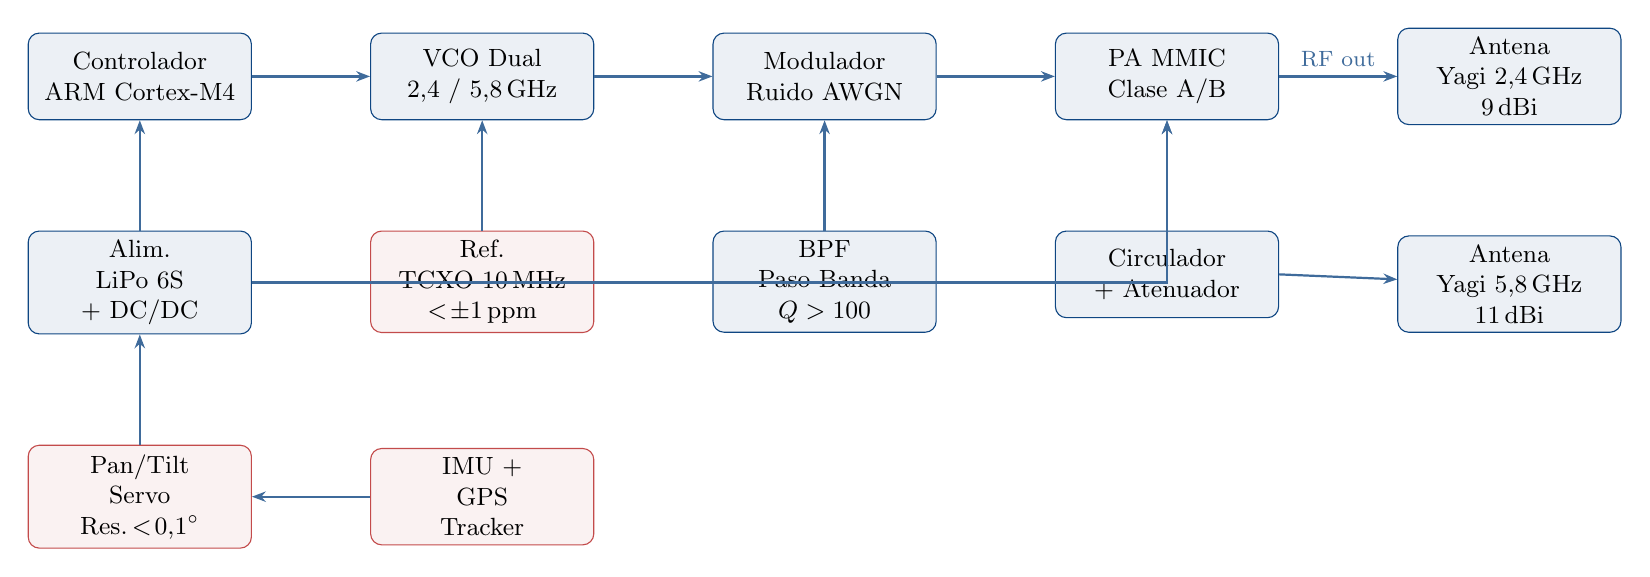
\begin{tikzpicture}[
  blk/.style  = {
    rectangle, draw=azultec, fill=azultec!8, rounded corners=4pt,
    text width=2.6cm, align=center, minimum height=1.1cm,
    font=\small
  },
  blkr/.style = {
    rectangle, draw=rojoalerta!80, fill=rojoalerta!6, rounded corners=4pt,
    text width=2.6cm, align=center, minimum height=1.1cm,
    font=\small
  },
  arr/.style  = {-{Stealth[length=5pt]}, thick, azultec!80},
  node distance = 1.5cm and 0.1cm
]

% Fila superior: cadena señal
\node[blk] (ctrl)  {Controlador\\ARM Cortex-M4};
\node[blk, right=1.5cm of ctrl] (vco)   {VCO Dual\\2,4 / 5,8\,GHz};
\node[blk, right=1.5cm of vco]  (mod)   {Modulador\\Ruido AWGN};
\node[blk, right=1.5cm of mod]  (pa)    {PA MMIC\\Clase A/B};
\node[blk, right=1.5cm of pa]   (ant24) {Antena\\Yagi 2,4\,GHz\\9\,dBi};

% Fila inferior: soporte
\node[blk,  below=1.4cm of ctrl] (psu)  {Alim.\\LiPo 6S\\+ DC/DC};
\node[blkr, below=1.4cm of vco]  (tcxo) {Ref.\\TCXO 10\,MHz\\\mbox{$<\!\pm1$\,ppm}};
\node[blk,  below=1.4cm of mod]  (bpf)  {BPF\\Paso Banda\\\mbox{$Q>100$}};
\node[blk,  below=1.4cm of pa]   (circ) {Circulador\\+ Atenuador};
\node[blk,  below=1.4cm of ant24](ant58){Antena\\Yagi 5,8\,GHz\\11\,dBi};

% Flechas cadena principal
\draw[arr] (ctrl)  -- (vco);
\draw[arr] (vco)   -- (mod);
\draw[arr] (mod)   -- (pa);
\draw[arr] (pa)    -- node[above,font=\footnotesize]{RF out} (ant24);
\draw[arr] (circ.east) -- (ant58);

% Flechas de soporte
\draw[arr] (psu.north)  -- (ctrl.south);
\draw[arr] (psu.east)  -| (pa.south);
\draw[arr] (tcxo.north) -- (vco.south);
\draw[arr] (bpf.north)  -- (mod.south);
\draw[arr] (circ.north) -- (pa.south);

% Etiqueta apuntado
\node[blkr, below=1.4cm of psu] (ptl) {Pan/Tilt\\Servo\\\mbox{Res.\,$<\!0{,}1^{\circ}$}};
\node[blkr, right=1.5cm of ptl] (imu) {IMU +\\GPS\\\mbox{Tracker}};
\draw[arr] (imu.west) -- (ptl.east);
\draw[arr] (ptl.north) -- (psu.south);

\end{tikzpicture}
\caption{Diagrama de bloques funcional — Sistema Soft Kill (jamming dual banda)}
\label{fig:bloques_sk}
\end{figure}

\subsubsection{Especificaciones de Componentes}

\begin{table}[H]
\centering
\caption{Especificaciones de componentes clave — Sistema Soft Kill}
\label{tab:comp_sk}
\renewcommand{\arraystretch}{1.25}
\begin{tabularx}{\textwidth}{lXX}
\toprule
\textbf{Componente} & \textbf{Especificación} & \textbf{Referencia comercial (ejemplo)} \\
\midrule
VCO dual banda &
  2.4 / 5.8\,GHz, ruido de fase $< -110$\,dBc/Hz @ 1\,MHz,
  ajuste $V_{tune}$ 0–5\,V &
  HMC507 (Analog Devices) \\[2pt]

Referencia de frecuencia &
  TCXO \SI{10}{MHz}, $|\Delta f/f| < \pm 1$\,ppm ($-40$\,a\,$+85\,^{\circ}$C) &
  TXC 7M-10.000MBE-T \\[2pt]

PA 2,4\,GHz (Banda S) &
  $P_\mathrm{sat} = 5$\,W (\SI{37}{dBm}), ganancia \SI{30}{dB},
  $P_{1\mathrm{dB}} > \SI{36}{dBm}$, eficiencia PAE $> 35\%$ &
  MAAP-011250 (MACOM) \\[2pt]

PA 5,8\,GHz (Banda C) &
  $P_\mathrm{sat} = 3$\,W (\SI{34.8}{dBm}), ganancia \SI{28}{dB} &
  SKY65453 (Skyworks) \\[2pt]

Antena 2,4\,GHz &
  Yagi 3 elementos, $G = 9$\,dBi, $Z_{in} = 50\,\Omega$,
  VSWR $< 1.5$, H-pol &
  Diseño propio (PCB FR4 / alu.) \\[2pt]

Antena 5,8\,GHz &
  Yagi 5 elementos, $G = 11$\,dBi, $Z_{in} = 50\,\Omega$ &
  Diseño propio \\[2pt]

Sustrato PCB RF &
  $\varepsilon_r = 3{,}5$, $\tan\delta = 0{,}0018$ @ \SI{10}{GHz},
  grosor 0,762\,mm &
  Taconic RF-35 \\[2pt]

Controlador de apuntado &
  ARM Cortex-M4 @ \SI{168}{MHz}, GPIO PWM 12\,bit,
  interfaz CAN/RS-485 &
  STM32F407 \\
\bottomrule
\end{tabularx}
\end{table}

\subsubsection{Diseño de PCB RF}

La placa de circuito impreso del módulo RF requiere las siguientes
consideraciones de diseño:

\begin{itemize}
  \item \textbf{Apilado de capas:}
        4 capas (señal RF — plano de masa — plano de alimentación — señal digital).
        Espesor total: \SI{1.6}{mm}.
  \item \textbf{Líneas de transmisión:}
        Microstrip $Z_0 = 50\,\Omega$ en capa~1 sobre plano de masa en capa~2.
        Para RF-35 ($\varepsilon_r = 3{,}5$, $h = 0{,}762$\,mm):
        ancho de pista $w \approx \SI{1.7}{mm}$.
  \item \textbf{Separación digital/RF:}
        Zonas de guarda (\textit{keepout}) alrededor de líneas RF.
        Vías de masa perimetrales cada $\lambda/20$ como mínimo.
  \item \textbf{Gestión térmica:}
        Pad térmico bajo el PA MMIC, vías térmicas al plano de cobre interno.
        Temperatura de unión máxima: $T_j < 150\,^{\circ}$C con $T_a = 55\,^{\circ}$C.
\end{itemize}

\newpage

% =====================================================================
\section{Sistema Hard Kill — Pulso Electromagnético de Alta Potencia}
% =====================================================================

\subsection{Mecanismos de Fallo en Electrónica Embarcada}

La interacción de un campo electromagnético intenso y rápidamente
variable con los circuitos integrados de un UAV puede producir
cuatro mecanismos de fallo diferenciados:

\begin{enumerate}[label=\textbf{\arabic*.}, leftmargin=*, itemsep=4pt]
  \item \textbf{Acoplamiento capacitivo en trazas de PCB.}
        El campo eléctrico incidente $\vec{E}$ induce tensiones parásitas
        proporcionales a $\mathrm{d}E/\mathrm{d}t$ en líneas de alta impedancia
        (entradas de ADC, lógica CMOS). Para trazas de longitud $\ell$ paralelas
        al campo, la tensión inducida es del orden de $V \sim E \cdot \ell$.

  \item \textbf{Inducción magnética en bucles de masa.}
        Según la ley de Faraday, un bucle de área $A$ expuesto a una variación
        $\partial B/\partial t$ genera una FEM:
        \[
          \mathcal{E} = -\frac{\mathrm{d}\Phi}{\mathrm{d}t}
                       = -A\,\frac{\partial B}{\partial t}
        \]
        Para un pulso de \SI{10}{ns} con $B_\mathrm{pico} = \SI{100}{\micro T}$
        y bucle de \SI{1}{cm^2}: $|\mathcal{E}| \approx \SI{10}{mV}$, suficiente
        para corromper lógica CMOS de \SI{3.3}{V} a través de ruido de modo común.

  \item \textbf{Avalancha en uniones p-n.}
        Las corrientes inducidas superan la tensión de ruptura inversa en diodos
        de protección ESD y transistores. El daño es \textbf{permanente e irreversible}.

  \item \textbf{Latch-up en CMOS.}
        Las corrientes transitorias activan el tiristor parásito (estructura pnpn)
        inherente en tecnología CMOS en bulk, creando un cortocircuito de
        baja impedancia entre $V_{DD}$ y GND. Puede ser destructivo si la
        fuente de alimentación no lo limita.
\end{enumerate}

\subsection{Umbrales de Susceptibilidad Electromagnética}

\begin{table}[H]
\centering
\caption{Umbrales de campo eléctrico para inducción de fallos en electrónica de UAVs}
\label{tab:umbrales}
\renewcommand{\arraystretch}{1.3}
\begin{tabularx}{\textwidth}{lXXl}
\toprule
\textbf{Tipo de dispositivo} &
\textbf{$E_\mathrm{min}$ (kV/m)} &
\textbf{Efecto observado} &
\textbf{Reversible} \\
\midrule
Receptor GNSS (módulo desnudo)  & 0,1–1   & Pérdida de \textit{fix}, trama NMEA corrupta & Sí \\
Receptor 2,4/5,8\,GHz          & 0,5–5   & Pérdida de enlace, reinicio receptor          & Sí \\
Microcontrolador CMOS sin blind.& 1–10    & Reset, corrupción de flash/RAM                & Sí/No \\
ESC (\textit{motor controller}) & 5–20    & Fallo de conmutación MOSFET                   & No \\
IMU (giróscopo MEMS)            & 10–50   & Saturación, fallo permanente del MEMS         & No \\
Módulo FPV transmisor           & 5–15    & Destrucción PA integrado                      & No \\
Electrónica con blindaje Al 1mm & 50–200  & Depende de rendijas y continuidad del shield  & No \\
Sistema mil. MIL-STD-461G       & ${>}500$& Diseño reforzado por especificación           & N/A \\
\bottomrule
\end{tabularx}
\end{table}

\subsection{Densidad de Potencia y Campo Eléctrico Requerido}

De la relación~\eqref{eq:poynting_media}, la densidad de potencia necesaria
para alcanzar un campo eléctrico umbral $E_\mathrm{min}$ es:

\begin{equation}
  S_\mathrm{req} = \frac{E_\mathrm{min}^2}{2\,Z_0}
  \label{eq:s_req}
\end{equation}

\begin{table}[H]
\centering
\caption{Densidad de potencia requerida por nivel de campo eléctrico ($Z_0 = \SI{377}{\ohm}$)}
\label{tab:s_campo}
\renewcommand{\arraystretch}{1.3}
\begin{tabularx}{\textwidth}{XXXX}
\toprule
$E_\mathrm{min}$ &
$S_\mathrm{req}$ (\si{W/m^2}) &
$S_\mathrm{req}$ (dBW/m²) &
Objetivo afectado \\
\midrule
\SI{1}{kV/m}   & $1{,}33 \times 10^3$ & $+31{,}2$ & GNSS, receptor RC \\
\SI{10}{kV/m}  & $1{,}33 \times 10^5$ & $+51{,}2$ & MCU, ESC sin blindaje \\
\SI{100}{kV/m} & $1{,}33 \times 10^7$ & $+71{,}2$ & Electrónica blindada \\
\SI{500}{kV/m} & $3{,}31 \times 10^8$ & $+85{,}2$ & Sistemas MIL \\
\bottomrule
\end{tabularx}
\end{table}

\subsection{Potencia de Pico Requerida por Distancia}

Combinando~\eqref{eq:densidad_antena} y~\eqref{eq:s_req}:

\begin{equation}
  P_\mathrm{pico} = \frac{S_\mathrm{req} \cdot 4\pi r^2}{G_t}
  \label{eq:ppico}
\end{equation}

La energía por pulso es $E_\mathrm{pulso} = P_\mathrm{pico} \cdot \tau$
y la energía almacenada en el banco, considerando eficiencia global
$\eta \approx 0{,}30$:

\begin{equation}
  E_C = \frac{E_\mathrm{pulso}}{\eta}
  \label{eq:ec}
\end{equation}

\begin{table}[H]
\centering
\caption{Potencia de pico y energía por pulso — Hard Kill ($E_\mathrm{min} = \SI{10}{kV/m}$,
         $G_t = \SI{20}{dBi}$, $\tau = \SI{10}{ns}$, $\eta = 0{,}30$)}
\label{tab:ppico}
\renewcommand{\arraystretch}{1.3}
\begin{tabularx}{\textwidth}{XXXXX}
\toprule
$r$ (m) &
$S_\mathrm{req}$ (W/m²) &
$P_\mathrm{pico}$ &
$E_\mathrm{pulso}$ &
$E_C$ (banco, $\eta = 0{,}30$) \\
\midrule
50   & $1{,}33 \times 10^5$ & \SI{83}{MW}    & \SI{0{,}83}{J} & \SI{2{,}8}{J}  \\
100  & $1{,}33 \times 10^5$ & \SI{333}{MW}   & \SI{3{,}3}{J}  & \SI{11}{J}     \\
200  & $1{,}33 \times 10^5$ & \SI{1{,}3}{GW} & \SI{13}{J}     & \SI{44}{J}     \\
500  & $1{,}33 \times 10^5$ & \SI{8{,}4}{GW} & \SI{84}{J}     & \SI{280}{J}    \\
\bottomrule
\end{tabularx}
\end{table}

\begin{notatec}
  La eficiencia global $\eta \approx 0{,}30$ engloba las pérdidas en:
  banco de condensadores ($\eta_C \approx 0{,}90$), red formadora de pulso
  ($\eta_\mathrm{PFN} \approx 0{,}80$), conmutador ($\eta_\mathrm{sw} \approx 0{,}85$)
  y antena + línea de transmisión ($\eta_\mathrm{ant} \approx 0{,}65$).
  El producto $0{,}90 \times 0{,}80 \times 0{,}85 \times 0{,}65 \approx 0{,}40$;
  un margen adicional de seguridad lleva el valor efectivo estimado a $\eta \approx 0{,}30$.
\end{notatec}

\subsection{Dimensionado de la Red Formadora de Pulso (PFN)}

Una PFN tipo Guillemin de $N$ secciones genera un pulso de forma
cuasirrectangular con duración $\tau$ e impedancia característica $Z_{PFN}$:

\begin{equation}
  \tau = 2\,\sqrt{L_\mathrm{total}\,C_\mathrm{total}}
  \qquad
  Z_{PFN} = \sqrt{\frac{L_\mathrm{total}}{C_\mathrm{total}}}
  \label{eq:pfn}
\end{equation}

\textbf{Diseño para $\tau = \SI{10}{ns}$, $Z_{PFN} = \SI{50}{\ohm}$:}

\begin{align}
  L_\mathrm{total} &= Z_{PFN}\cdot\frac{\tau}{2}
    = 50 \times \frac{10\times10^{-9}}{2} = \SI{250}{nH} \\[4pt]
  C_\mathrm{total} &= \frac{\tau}{2\,Z_{PFN}}
    = \frac{10\times10^{-9}}{100} = \SI{100}{pF}
\end{align}

Para una PFN de $N=5$ secciones: $L_k = \SI{50}{nH}$,
$C_k = \SI{20}{pF}$ por sección.

\subsection{Dimensionado del Banco de Condensadores}

La energía almacenada en el banco:

\begin{equation}
  E_C = \frac{1}{2}\,C_\mathrm{banco}\,V_0^2
  \label{eq:banco}
\end{equation}

Para objetivo en $r = \SI{200}{m}$ ($E_C = \SI{44}{J}$) con $V_0 = \SI{10}{kV}$:

\begin{equation}
  C_\mathrm{banco} = \frac{2\,E_C}{V_0^2}
                   = \frac{2 \times 44}{(10^4)^2}
                   = \SI{0{,}88}{\micro F}
                   \approx \SI{1}{\micro F}
\end{equation}

Con margen de diseño del 50\% y degradación de capacitancia a largo plazo,
se especifica $C_\mathrm{banco} = \SI{2}{\micro F}$ @ \SI{15}{kV}.

\subsection{Arquitectura del Sistema Hard Kill}

\begin{figure}[H]
\centering
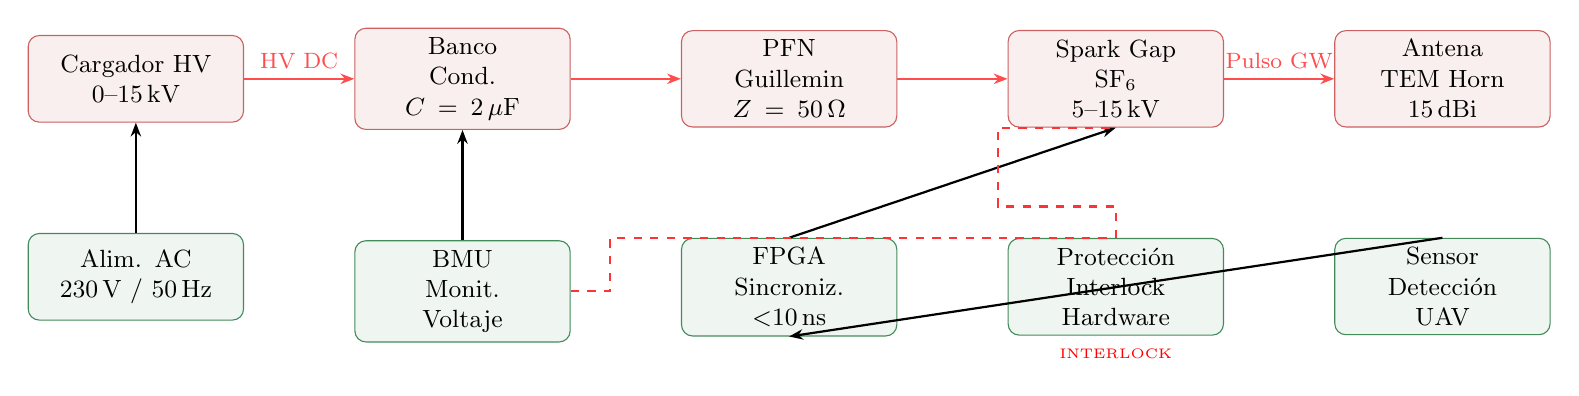
\begin{tikzpicture}[
  blk/.style  = {
    rectangle, draw=rojoalerta!70, fill=rojoalerta!7,
    rounded corners=4pt, text width=2.5cm, align=center,
    minimum height=1.1cm, font=\small
  },
  blkg/.style = {
    rectangle, draw=verdecorrec!80, fill=verdecorrec!7,
    rounded corners=4pt, text width=2.5cm, align=center,
    minimum height=1.1cm, font=\small
  },
  arr/.style  = {-{Stealth[length=5pt]}, thick},
  harr/.style = {-{Stealth[length=5pt]}, thick, red!70},
  node distance = 1.6cm and 0.1cm
]

% Cadena principal (fila superior)
\node[blk]                       (hvps) {Cargador HV\\0–15\,kV};
\node[blk, right=1.4cm of hvps]  (cap)  {Banco\\Cond.\\$C=\SI{2}{\mu F}$};
\node[blk, right=1.4cm of cap]   (pfn)  {PFN\\Guillemin\\$Z=\SI{50}{\ohm}$};
\node[blk, right=1.4cm of pfn]   (sg)   {Spark Gap\\SF$_6$\\5–15\,kV};
\node[blk, right=1.4cm of sg]    (tem)  {Antena\\TEM Horn\\15\,dBi};

% Fila soporte inferior
\node[blkg, below=1.4cm of hvps] (ac)   {Alim. AC\\230\,V / 50\,Hz};
\node[blkg, below=1.4cm of cap]  (bmu)  {BMU\\Monit.\\Voltaje};
\node[blkg, below=1.4cm of pfn]  (fpga) {FPGA\\Sincroniz.\\$<$\SI{10}{ns}};
\node[blkg, below=1.4cm of sg]   (prot) {Protección\\Interlock\\Hardware};
\node[blkg, below=1.4cm of tem]  (radar){Sensor\\Detección\\UAV};

% Flechas cadena principal
\draw[harr] (hvps) -- node[above,font=\footnotesize]{HV DC} (cap);
\draw[harr] (cap)  -- (pfn);
\draw[harr] (pfn)  -- (sg);
\draw[harr] (sg)   -- node[above,font=\footnotesize]{Pulso GW} (tem);

% Flechas soporte
\draw[arr] (ac)    -- (hvps);
\draw[arr] (bmu.north)  -- (cap.south);
\draw[arr] (fpga.north) -- (sg.south);
\draw[arr] (radar.north) -- (fpga.south);

% Interlock (línea discontinua roja)
\draw[dashed, red!80, thick] (bmu.east) -- ++(0.5,0) |- (prot.north);
\draw[dashed, red!80, thick] (prot.north) -- ++(0,0.4) -- ++(-1.5,0) |- (sg.south);
\node[font=\tiny, red, below=0.05cm of prot] {INTERLOCK};

\end{tikzpicture}
\caption{Diagrama de bloques funcional — Sistema Hard Kill (pulso HPM)}
\label{fig:bloques_hk}
\end{figure}

\subsubsection{Especificaciones de Componentes — Hard Kill}

\begin{table}[H]
\centering
\caption{Especificaciones de componentes clave — Sistema Hard Kill}
\label{tab:comp_hk}
\renewcommand{\arraystretch}{1.25}
\begin{tabularx}{\textwidth}{lXX}
\toprule
\textbf{Componente} & \textbf{Especificación} & \textbf{Notas de diseño} \\
\midrule
Condensadores de pulso &
  \SI{1}{\micro F} @ \SI{15}{kV} pp,
  ESR $< \SI{5}{m\ohm}$, ESL $< \SI{50}{nH}$,
  vida $> 10^6$ ciclos &
  Polipropileno metalizado o mica. Montaje en paralelo para
  reducir ESL efectiva. \\[4pt]

Spark gap SF$_6$ presurizado &
  $V_\mathrm{ruptura}$ ajustable 5–15\,kV,
  jitter $< \SI{1}{ns}$,
  vida $> 10^6$ disparos,
  $t_\mathrm{cond} < \SI{100}{ps}$ &
  Presión SF$_6$ ajusta $V_\mathrm{ruptura}$.
  Disparo por láser o pulso de trigatrón opcional. \\[4pt]

PFN Guillemin (5 sec.) &
  $Z = \SI{50}{\ohm}$, $\tau = \SI{10}{ns}$,
  $V_\mathrm{max} = \SI{15}{kV}$,
  $L_k = \SI{50}{nH}$, $C_k = \SI{20}{pF}$ &
  Inductores de aire o toroide ferrita saturada para
  alta potencia de pico. \\[4pt]

Antena TEM Horn &
  BW: 500\,MHz – 10\,GHz,
  $G = 12$–$15$\,dBi (pico),
  $Z_{in} = \SI{50}{\ohm}$,
  apertura $30 \times 30$\,cm &
  Alimentación balanceada mediante balun o transición
  coaxial–stripline. Refrigeración forzada. \\[4pt]

FPGA de sincronización &
  Latencia disparo $< \SI{10}{ns}$,
  E/S LVTTL 3,3\,V,
  reloj interno $\geq \SI{200}{MHz}$ &
  Artix-7 (Xilinx) o Cyclone~V (Intel).
  Código VHDL/Verilog para control de timing. \\[4pt]

Cargador HV &
  0–15\,kV, $\SI{200}{mA}$ máx.,
  control digital (SPI/I²C),
  aislamiento $\geq \SI{20}{kV}$ &
  Módulos apilables tipo flyback o SEPIC HV.
  Detección de cortocircuito en $< \SI{1}{\micro s}$.\\
\bottomrule
\end{tabularx}
\end{table}

\newpage

% =====================================================================
\section{Sistema de Detección y Apuntado}
% =====================================================================

\subsection{Comparativa de Modalidades de Detección}

\begin{table}[H]
\centering
\caption{Análisis comparativo de métodos de detección de UAVs}
\label{tab:deteccion}
\renewcommand{\arraystretch}{1.25}
\begin{tabularx}{\textwidth}{lXXXl}
\toprule
\textbf{Método} &
\textbf{Alcance} &
\textbf{Ventajas} &
\textbf{Limitaciones} &
\textbf{Coste relativo} \\
\midrule
Radar FMCW &
  0,1–5\,km &
  Alta precisión en rango y velocidad, todo tiempo, activo &
  Requiere licencia de espectro, alta complejidad &
  Alto \\[3pt]

Detector RF pasivo &
  0,1–2\,km &
  Sin emisión, detecta enlace RC / telemetría &
  Ciego si UAV en modo autónomo (GNSS only) &
  Medio \\[3pt]

Array de micrófonos &
  50–500\,m &
  Pasivo, sin emisión, bajo coste &
  Afectado por ruido ambiental, viento &
  Bajo \\[3pt]

Visión + IA (EO/IR) &
  50\,m–1\,km &
  Identificación visual, integración IA &
  Niebla, lluvia, contraluz, noche (solo IR) &
  Medio \\[3pt]

LIDAR 3D &
  50–500\,m &
  Alta resolución de nube de puntos &
  Alcance limitado, sensible a lluvia/polvo &
  Alto \\[3pt]

Fusión (radar+RF+EO) &
  0,1–3\,km &
  Máxima robustez, mínimos falsos positivos &
  Coste y complejidad de integración &
  Muy alto \\
\bottomrule
\end{tabularx}
\end{table}

\begin{notatec}
  La solución recomendada para el prototipo de laboratorio es la
  combinación \textbf{detector RF pasivo + cámara EO} por relación
  coste-prestaciones. El FMCW radar se contempla en la fase de
  pre-producción para entornos operativos exigentes.
\end{notatec}

\subsection{Requisitos del Sistema de Apuntado}

El ancho de haz a \SI{-3}{dB} de una antena de apertura $D$
a frecuencia $f$ es:

\begin{equation}
  \theta_{3\mathrm{dB}} \approx \frac{70\,\lambda}{D} \quad [\text{grados}]
  \label{eq:haz}
\end{equation}

Para la antena TEM Horn con apertura $D = \SI{30}{cm}$
y frecuencia central $f = \SI{3}{GHz}$ ($\lambda = \SI{100}{mm}$):

\begin{equation}
  \theta_{3\mathrm{dB}} \approx \frac{70 \times 0{,}10}{0{,}30} \approx 23^{\circ}
\end{equation}

Esto implica que el servo de apuntado debe mantener el haz centrado
en el UAV con un error $\leq 10^{\circ}$ para garantizar una caída de ganancia
$< 3$\,dB. Los requisitos del sistema de apuntado son:

\begin{itemize}[noitemsep]
  \item Velocidad angular máxima: $\geq 90^{\circ}$/s (azimut y elevación)
  \item Resolución angular: $\leq 0{,}1^{\circ}$ (encoder absoluto de $\geq 12$\,bits)
  \item Rango de movimiento: azimut $\pm 180^{\circ}$, elevación $0^{\circ}$–$90^{\circ}$
  \item Par mínimo: función de la masa del cabezal EM (estimado \SI{5}{N\cdot m})
  \item Latencia lazo de control: $< \SI{10}{ms}$
\end{itemize}

\newpage

% =====================================================================
\section{Marco Regulatorio}
% =====================================================================

\begin{table}[H]
\centering
\caption{Marco regulatorio aplicable — Sistemas C-UAS electromagnéticos}
\label{tab:regulatorio}
\renewcommand{\arraystretch}{1.25}
\begin{tabularx}{\textwidth}{llX}
\toprule
\textbf{Norma / Regulación} &
\textbf{Ámbito} &
\textbf{Implicación para el sistema} \\
\midrule
ITU-R SM.329-12 &
  Internacional &
  Límites de emisiones fuera de banda y espurias \\[3pt]

ITU Radio Reglamento, Art.~15 &
  Internacional &
  Prohibición expresa de interferencia a otros servicios
  radioeléctricos \\[3pt]

ETSI EN 303 413 &
  UE &
  Requisitos de compatibilidad EM para equipos GNSS \\[3pt]

Directiva 2014/53/UE (RED) &
  UE &
  Homologación de equipos radio en el mercado europeo \\[3pt]

EASA Regl. 2019/947 y 2021/664 &
  UE &
  Marco de operación de UAVs y sistemas C-UAS en espacio aéreo civil \\[3pt]

Ley 9/2014 General de Telecom. &
  España &
  Gestión del espectro radioeléctrico y sanciones por interferencia \\[3pt]

CNAF (Cuadro Nacional de AF) &
  España &
  Asignación de frecuencias; uso de bandas 2,4 / 5,8\,GHz (ISM) \\[3pt]

MIL-STD-461G &
  Defensa EE.UU. &
  Requisitos de compatibilidad EM para equipos militares \\[3pt]

STANAG 4370 — AECTP 500 &
  OTAN &
  Procedimientos de ensayo EM ambiental \\[3pt]

FCC Part 15 / 47 C.F.R. §97 &
  EE.UU. &
  Aplicable si se comercializa en EE.UU.; importaciones sujetas a
  aprobación FCC \\
\bottomrule
\end{tabularx}
\end{table}

\begin{correccion}[Aviso Legal Crítico]
  El despliegue de sistemas de \textbf{jamming activo} (Soft Kill) y
  de \textbf{HPM} (Hard Kill) en espacio aéreo civil está
  \textbf{prohibido} sin autorización expresa de la administración
  nacional de telecomunicaciones (en España: CNMC / SETELCO).
  En la mayoría de jurisdicciones, el uso está exclusivamente reservado
  a Fuerzas y Cuerpos de Seguridad del Estado y Fuerzas Armadas,
  previa habilitación de espectro.
  El desarrollo de prototipos requiere coordinación con la AESA
  (Agencia Estatal de Seguridad Aérea) para pruebas de campo.
\end{correccion}

\newpage

% =====================================================================
\section{Plan de Desarrollo Industrial}
% =====================================================================

\subsection{Fases del Proyecto y Entregables}

\begin{table}[H]
\centering
\caption{Cronograma de desarrollo — Hitos y criterios de éxito}
\label{tab:cronograma}
\renewcommand{\arraystretch}{1.3}
\begin{tabularx}{\textwidth}{lXXX}
\toprule
\textbf{Fase} &
\textbf{Duración} &
\textbf{Entregables} &
\textbf{Criterio de éxito} \\
\midrule
1. Diseño Conceptual &
  3 meses &
  Especificación técnica v1.0;
  simulaciones EM en HFSS/CST;
  selección de componentes &
  Validación de arquitectura por revisión técnica interna \\[4pt]

2. Prototipo de Laboratorio &
  6 meses &
  PCB RF funcional (Soft Kill);
  banco de condensadores de prueba;
  SW de control v0.1 &
  Medición de parámetros en cámara anecoica;
  verificación de potencia de salida RF \\[4pt]

3. Integración y Pruebas de Campo &
  9 meses &
  Sistema integrado en plataforma trípode;
  sistema de apuntado operativo;
  ensayos contra UAV de prueba homologado &
  Neutralización efectiva en $\geq 80\%$ de intentos
  en rango $\leq \SI{200}{m}$ \\[4pt]

4. Prototipo Pre-serie &
  6 meses &
  5 unidades pre-serie;
  documentación técnica completa (ICD, BOM, BoM);
  ensayos MIL-STD-461 &
  Superación de ensayos EMC y ambientales \\[4pt]

5. Producción en Serie &
  Continuo &
  Lotes de 10–50 unidades;
  soporte técnico y formación &
  Tasa de rechazo en producción $< 2\%$;
  MTBF $> \SI{2000}{h}$ \\
\bottomrule
\end{tabularx}
\end{table}

\subsection{Estimación de Costes}

\begin{table}[H]
\centering
\caption{Estimación de costes unitarios de producción (escala $\geq 50$ unidades)}
\label{tab:costes}
\renewcommand{\arraystretch}{1.3}
\begin{tabularx}{\textwidth}{lXX}
\toprule
\textbf{Subsistema} &
\textbf{Coste unitario (USD)} &
\textbf{Observaciones} \\
\midrule
Módulo RF Soft Kill (dual banda 2,4/5,8\,GHz) &
  2.500–4.500 &
  Incluye PCB RF 4 capas, PA MMIC $\times 2$, antenas Yagi, drivers \\[3pt]

Módulo GNSS Jamming (L1/L2) &
  500–1.500 &
  Circuitería adicional; muy bajo coste por baja potencia requerida \\[3pt]

Módulo Hard Kill (PFN + Spark Gap + TEM Horn) &
  18.000–35.000 &
  Condensadores de pulso representan $\approx 40\%$ del coste \\[3pt]

Sistema de apuntado (pan/tilt + encoders + servos) &
  3.000–6.000 &
  Servos industriales; encoder absoluto 14\,bit \\[3pt]

Unidad de control (FPGA + ARM + HMI) &
  2.500–5.000 &
  Pantalla táctil 7'', conectividad Ethernet/CAN \\[3pt]

Chasis y mecánica (aluminio, IP54) &
  2.000–4.000 &
  Anodizado, juntas de estanqueidad, quick-release antenas \\[3pt]

Sistema de alimentación (batería + BMS + cargador) &
  1.500–3.000 &
  LiPo 6S + cargador HV independiente \\[3pt]

\midrule
\textbf{Coste total de fabricación (COGS)} &
  \textbf{30.000–59.000} &
  Sin margen comercial ni ingeniería \\[2pt]

\textbf{PVP estimado (margen $2{,}5\times$)} &
  \textbf{75.000–148.000} &
  Mercado de defensa / seguridad pública \\[2pt]

\textbf{PVP Solo Soft Kill (sin Hard Kill)} &
  \textbf{20.000–40.000} &
  Versión reducida para mercado policial \\
\bottomrule
\end{tabularx}
\end{table}

\newpage

% =====================================================================
\section*{Conclusiones y Próximos Pasos}
\addcontentsline{toc}{section}{Conclusiones y Próximos Pasos}
% =====================================================================

\subsection*{Conclusiones Técnicas}

\begin{enumerate}[itemsep=4pt]
  \item El \textbf{jamming de banda 2,4\,GHz} a \SI{500}{m} requiere
        $\sim\SI{1}{W}$ de potencia transmitida con antena Yagi de 9\,dBi
        y margen de jamming de 15\,dB. Los PA MMIC comerciales disponibles
        cubren esta especificación sin dificultad.

  \item La \textbf{neutralización GNSS} ($r \leq \SI{2}{km}$) es técnicamente
        trivial en términos de potencia ($< \SI{35}{mW}$), pero presenta el
        mayor riesgo regulatorio y colateral del sistema.

  \item El módulo \textbf{Hard Kill} para $r = \SI{200}{m}$ requiere un banco
        de condensadores de $\approx \SI{2}{\micro F}$ a \SI{10}{kV}
        (energía almacenada $\approx \SI{100}{J}$), dimensiones alcanzables
        con tecnología comercial de condensadores de pulso de polipropileno.

  \item La \textbf{antena TEM Horn} es la solución óptima para HPM por su
        ancho de banda ultraamplio (500\,MHz–10\,GHz), capacidad de
        manejar potencias de GW en pulso y patrón de radiación controlado.

  \item El \textbf{coste dominante} del sistema integrado son los
        condensadores de pulso de alta tensión y el módulo de HV, que
        representan $\sim 60\%$ del COGS del subsistema Hard Kill.
\end{enumerate}

\subsection*{Próximos Pasos Inmediatos}

\begin{itemize}[itemsep=3pt]
  \item[$\square$] Simulación EM de la antena Yagi 2,4\,GHz en CST Microwave Studio
        (verificación de ganancia, diagrama de radiación y VSWR).
  \item[$\square$] Diseño esquemático detallado del módulo RF
        (VCO + PA + BPF + circulador) y layout de PCB en Altium Designer.
  \item[$\square$] Pedido de muestras de condensadores de pulso
        (p.\,ej., Murata RDER-series o Cornell Dubilier 942C-series).
  \item[$\square$] Evaluación de spark gaps comerciales (p.\,ej., Perkin-Elmer
        GP15 o PerkinElmer N21AF) y prueba de jitter.
  \item[$\square$] Consulta legal con asesor especializado en regulación
        de espectro y defensa (CNMC, AESA, Ministerio de Defensa) sobre
        marco de autorización para pruebas de campo.
  \item[$\square$] Definición de protocolo de ensayo en cámara anecoica
        (rango 1–10\,GHz, validación de PIRE real vs. calculado).
\end{itemize}

% =====================================================================
\begin{thebibliography}{10}

\bibitem{balanis}
  C.\,A. Balanis,
  \textit{Antenna Theory: Analysis and Design}, 4.ª\,ed.
  Wiley, 2016.

\bibitem{pozar}
  D.\,M. Pozar,
  \textit{Microwave Engineering}, 4.ª\,ed.
  Wiley, 2011.

\bibitem{griffiths}
  D.\,J. Griffiths,
  \textit{Introduction to Electrodynamics}, 4.ª\,ed.
  Cambridge University Press, 2017.

\bibitem{ott}
  H.\,W. Ott,
  \textit{Electromagnetic Compatibility Engineering}.
  Wiley, 2009.

\bibitem{wik}
  M. Wik, A. Rybachevsky, A. Weinachter,
  ``Electromagnetic Susceptibility of Consumer Electronics,''
  \textit{IEEE Trans. Electromagn. Compat.}, vol.~54, no.~4, pp.~830–838, 2012.

\bibitem{nato_cuas}
  NATO STO,
  \textit{Counter-UAS Systems: Technology Survey and Roadmap},
  TR-SET-232, 2021.

\bibitem{itu_sm329}
  ITU-R,
  \textit{Recommendation SM.329-12: Unwanted emissions in the spurious domain},
  Ginebra, 2012.

\bibitem{milstd461}
  U.S. Department of Defense,
  \textit{MIL-STD-461G: Requirements for the Control of Electromagnetic
  Interference Characteristics of Subsystems and Equipment}, 2015.

\bibitem{pfn_theory}
  J.\,C. Martin,
  \textit{Nanosecond Pulse Techniques} (AWRE Report).
  UCRL-ID-110173, Lawrence Livermore National Laboratory, 1992.

\bibitem{tem_horn}
  D.\,V. Giri, F.\,M. Tesche,
  ``Classification of Intentional Electromagnetic Environments (IEME),''
  \textit{IEEE Trans. Electromagn. Compat.}, vol.~46, no.~3, pp.~322–328, 2004.

\end{thebibliography}

\end{document}